\begin{figure}[!htb]
    \centering
    \begin{subfigure}{0.49\textwidth}
        \centering
        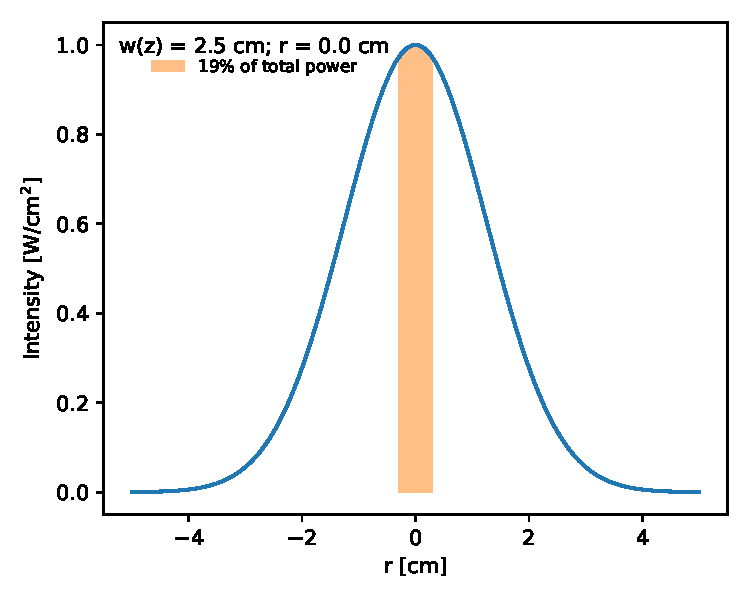
\includegraphics[width=1\textwidth]{figures/measurements/power-curve-453GHz/beam_propagation_power_curve_w0-2.50_offset-0.00_dia-0.60.pdf}
        \caption{}
        \label{fig:power-curve:beam-propagation-power:at0}
    \end{subfigure}
    \hfill
    \begin{subfigure}{0.49\textwidth}
        \centering
        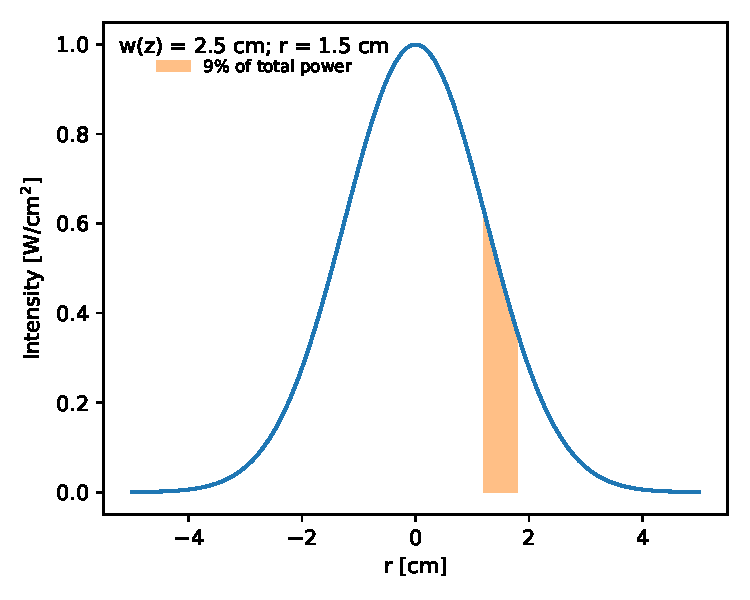
\includegraphics[width=1\textwidth]{figures/measurements/power-curve-453GHz/beam_propagation_power_curve_w0-2.50_offset-1.50_dia-0.60.pdf}
        \caption{}
        \label{fig:power-curve:beam-propagation-power:offset}
    \end{subfigure}
    \caption{The radiation intensity profile distribution is shown in the blue line. The shaded orange region indicates the fraction of output power at a 3 cm beam radius, i.e., inside trap region as shown in Figure \ref{fig:power-curve:beam-propagation}. The position of the orange region \emph{w.r.t} the x-axis represents the part of the propagating Gaussian beam reaching the trap region when (a): aligned and (b): 1.5 cm offset \emph{w.r.t} beam centre.}
    \label{fig:power-curve:beam-propagation-power}
\end{figure}
